
\begin{frame}
\frametitle{Baseline: motivación}
Busco fijar el setup de entrenamiento con valores razonables \pause
\begin{itemize}
\item El feature set va a cambiar cada experimento \pause
\item El dataset está fijo \pause
\item El método de entrenamiento principal es \textit{target scores} \pause
\end{itemize}
Entonces queda por determinar\dots
\begin{itemize}
\item La arquitectura de la red ($L_1$ y $L_2$) \pause
\item Los hiperparámetros
\end{itemize}
\end{frame}


\begin{frame}
\frametitle{Baseline: hiperparámetros}
Los hiperparámetros fueron seleccionados en base al trainer oficial de Stockfish: \pause
\begin{itemize}
\item \textbf{Learning rate}: 0.0005 \pause
\item \textbf{Exponential decay}: 0.99 \pause
\item \textbf{Batch size}: 16384 \pause
\item \textbf{Epoch size}: 100 million \pause
\begin{itemize}
    \item cada epoch realiza 6104 batches \pause
\end{itemize}
\item \textbf{Epochs}: 256
\begin{itemize}
    \item cada run observa \textit{25.6 billion} samples
\end{itemize}
\end{itemize}
\end{frame}


\begin{frame}
\frametitle{Baseline: experimento}
Sólo queda buscar parámetros $L_1$ y $L_2$ razonables. Realizo una búsqueda en grilla con:
\begin{itemize}
\item L1 $\in \{256, 512, 1024, 2048\}$
\item L2 $\in \{32, 64, 128, 256\}$
\end{itemize}
El feature set a utilizar es \featureset{All}[768].
\end{frame}

\begin{frame}
\frametitle{Baseline: resultados}
\begin{figure}
\centering
\makebox[\textwidth]{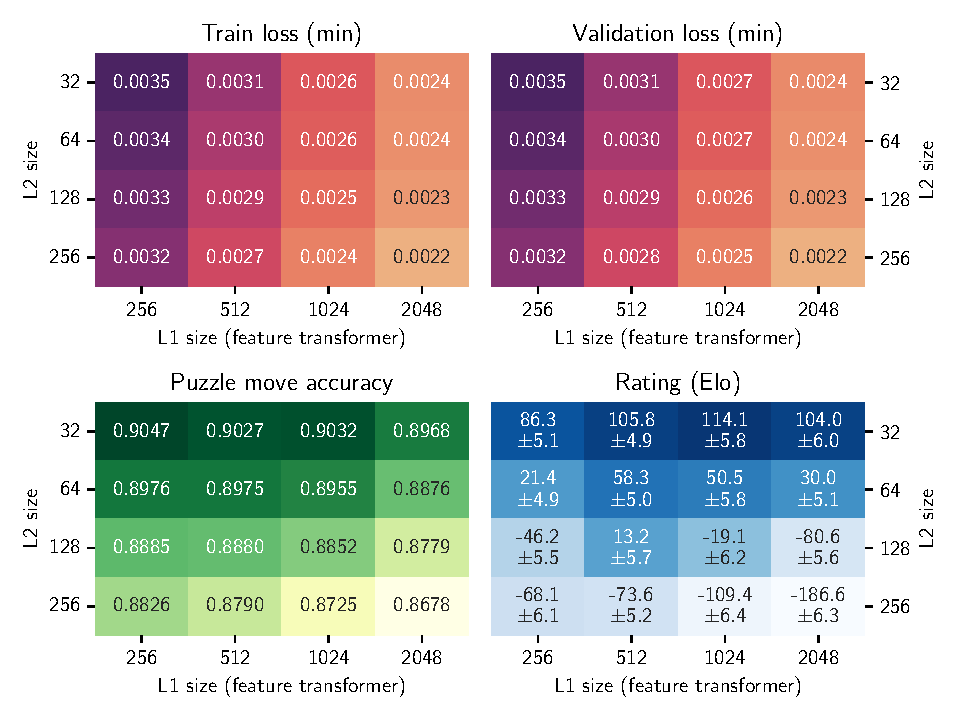
\includegraphics[width=0.93\textwidth]{../thesis/dynamic/output/baseline_heatmaps.pdf}}
\end{figure}
\end{frame}

\begin{frame}
\frametitle{Baseline: conclusión}
\begin{itemize}
\item \textbf{L2=32}. El performance cae dramáticamente si L2 aumenta, utilizo el más bajo.
\begin{itemize}
    \item Sería buena idea probar valores más chicos de L2. \pause
\end{itemize}
\item \textbf{L1=512}. Es el mejor valor para L2=64 y L2=128, y en margen de error para L2=32.
\begin{itemize}
    \item Además es el más rápido de entrenar.
\end{itemize}
\end{itemize}
\end{frame}
